\section{861 - Little bishops}

\textbf{Problema:} dados dos enteros $n$ y $k$, devolver la cantidad
de formas de ubicar $k$ alfiles en un tablero de $n \times n$, de manera tal
que ninguno de ellos sea atacado por otro.

\subsection{Resoluci\'on}
Para resolverlo, primero notamos que las casillas negras y las blancas
son independientes, en el sentido de que un alfil en una casilla de un color
nunca puede atacar a un alfil en una casilla del color opuesto.
Por esta raz\'on, la cantidad de formas de ubicar $k$ alfiles
en un tablero de $n \times n$ se puede calcular de la siguiente manera:

Sea $a_k$ la cantidad de formas de ubicar $k$ alfiles sin que se ataquen
en un tablero de $n \times n$. Si $a_k^B$ es la cantidad de formas de ubicar 
$k$ alfiles sin que se ataquen en las casillas blancas y
$a_k^N$ es la cantidad de formas de hacerlo en las negras, entonces vale que:

$$a_k = \sum_{i=0}^k{a_i^N \cdot a_{k-i}^B}$$

Por otro lado, mirando s\'olo las casillas negras 
(es an\'alogo para las blancas) y rotando el tablero $45�$, 
el problema de ubicar alfiles se puede interpretar como un
problema de ubicar torres.

\begin{figure}[H]
\centering
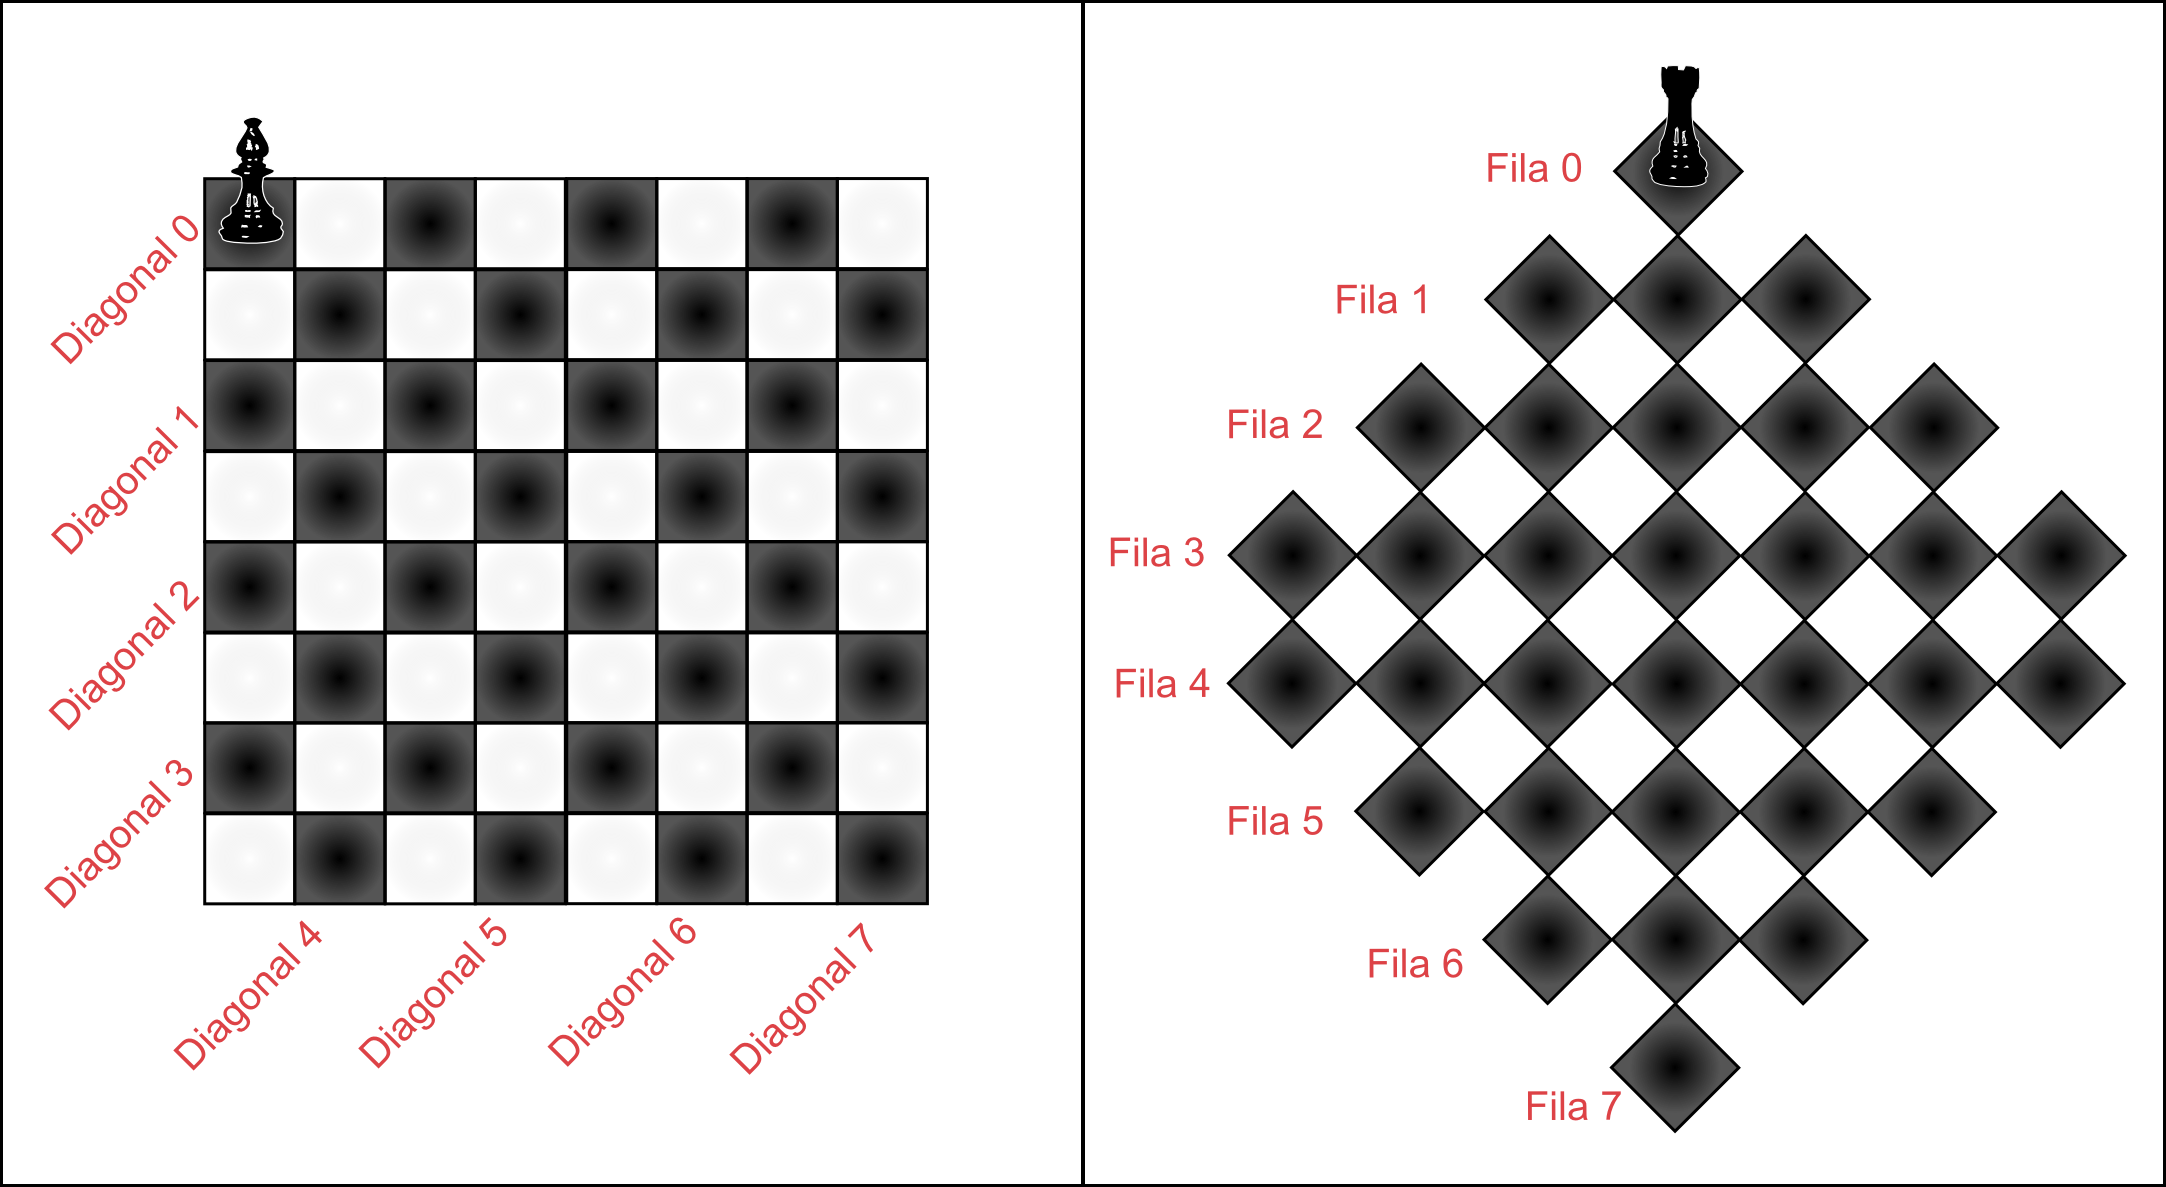
\includegraphics[scale=0.30]{./figuras/tablero1.png}
\caption{Interpretaci\'on del problema de los alfiles como uno de torres}
\end{figure}

Consideramos ahora el problema de ubicar torres, sin que se ataquen,
en un tablero de varias filas, cada una de las cuales puede tener un
n\'umero diferente de columnas.
Es f\'acil ver que a lo sumo puede haber una torre por fila, y que
permutar filas no modifica la cantidad de torres que se pueden ubicar. 
Sea $columnas(i)$ la cantidad de columnas de la fila $i$.
Si se ordenan las filas crecientemente por su cantidad de columnas,
vale que las columnas de cada fila 
est�n incluidas en las de las filas que est�n abajo. Esto quiere 
decir que, al ubicar una torre, la columna en la que fue ubicada queda
inutilizable para las filas siguientes.

A partir de esto podemos definir la siguiente recurrencia:

Sea $cantidad(i,j)=$ cantidad de formas de poner $j$ torres usando las 
primeras $i$ filas (ordenadas crecientemente por cantidad de columnas). Vale entonces 
que:

$cantidad(i,0) = 1 $, porque hay solo una forma de no poner ninguna torre.

$cantidad(0,j) = 0  \ si \ j > 0$, porque no hay forma de poner alguna torre si no quedan casillas.
 
$cantidad(i,j) = cantidad(i-1,j) + cantidad(i-1,j-1) \cdot (columnas(i)-(j-1))\ si \ i > 0$, 
porque o bien se ponen las $j$ torres en la filas anteriores, o bien se pone una en 
la fila actual y el resto en las anteriores. Al hacer eso, se est\'an ocupando $j-1$ 
columnas; las restantes quedan libres, por lo cual para cada posible forma de ubicar 
las torres en las anteriores filas hay $columnas(i) - (j-1)$ columnas libres que 
pueden usarse.

Aplicamos la resoluci\'on del problema de ubicar torres sobre las diagonales
negras y las diagonales blancas, para as\'i calcular $a^N_k$ y $a^B_k$.
Pueden hacerse las siguientes optimizaciones:
\begin{itemize}
\item No es necesario ``ordenar'' las diagonales, basta con notar que para las
casillas negras las longitudes de las diagonales son 1, 1, 3, 3, ..., etc. (para
las casillas blancas es similar pero empezando desde 2).

\item Si $n$ es par, las casillas blancas y las negras son sim\'etricas,
por lo cual la cantidad de formas de ubicar las piezas es la misma para
unas y otras (es decir, $a^B_k = a^N_k$). En ese caso, basta con resolver
el problema para las casillas de uno de los colores.

\item Si $n > 1$, la cantidad m\'axima de alfiles que se pueden poner en un tablero de $n \times n$ es $2n - 2$.
Esto es porque hay $2n - 1$ diagonales pero adem\'as no pueden ubicarse dos alfiles en esquinas opuestas\footnote{
Adem\'as est\'a demostrado: 

Dudeney, H. E. ``Bishops--Unguarded'' and ``Bishops--Guarded.'' \S 297 and 298 in Amusements in Mathematics. New York: Dover, pp. 88-89 and 96, 1970.

Madachy, J. Madachy's Mathematical Recreations. New York: Dover, pp. 36-46, 1979. }
con lo cual si el $k$ ingresado es mayor, se puede devolver 0 sin procesar nada.

\item En todas las diagonales de un color, se pueden poner a lo sumo $n - 1$ alfiles, esto es f�cil de ver, si consideramos un tablero ubicado como el de la figura, las casillas negras tienen $n$ diagonales ascendentes, pero dos son de una sola casilla y est�n en la misma diagonal descendente. Si $n$ es par las casillas blancas son sim�tricas a las negras, por lo que la cantidad de alfiles que se pueden ubicar es la misma. Si en cambio $n$ es impar, hay $n-1$ diagonales blancas ascendentes, que a lo sumo pueden tener un alfil cada una.
Es por esta raz�n que no hace falta hacer la sumatoria desde $0$ hasta $k$, sino que se puede hacer
desde $max(0, k - (n - 1))$ hasta $min(k, n - 1)$. Esto s\'olo vale si $n > 1$, ya que con $n = 1$
no hay casillas blancas.
\end{itemize}

En base a la recurrencia planteada, se ve que basta con llenar una matriz $M$ de $(n + 1) \times (k + 1)$
para las negras y otra para las blancas, de modo que $M[i][j]=cantidad(i,j)$. El siguiente es el
algoritmo de llenado de la tabla para las casillas negras. Si el tablero es impar, el algoritmo
para las casillas blancas es similar. Dado que en cada paso s\'olo se necesita la fila anterior,
en la implementaci\'on la matriz se representa guardando s\'olo las \'ultimas dos filas,
cada una de $k + 1$ elementos.

\begin{algorithm}[H]
\begin{algorithmic}
\caption{\texttt{ubicar\_en\_negras}: maneras de ubicar $\leq k$ alfiles en las casillas negras de un tablero de $n \times n$}
\PARAMS{$n$: alto del tablero, $k$: m\'axima cantidad de alfiles que se quieren poner}
\STATE $M$ := matriz de $(n + 1)$ filas y  $(k+1)$ columnas %%tal que $M_{ij}=0$
%\STATE\COMMENT{$M_{i,j}$ = cantidad de maneras de poner $j$ alfiles en las diagonales negras $[0,i)$}
\STATE $M_{i,0} := 1$ para todo $i$
\STATE $M_{0,j} := 0$ para todo $j > 0$
\FOR{cada $i$ en $[1,n]$}
	\STATE $casillas$ := n\'umero de casillas de la $(i - 1)$-\'esima diagonal negra
	\FOR{cada $j$ en $[1,k]$}
		\STATE $M_{i,j} := M_{i-1,j} + M_{i-1,j-1}*(casillas - (j-1))$
	\ENDFOR
\ENDFOR
\STATE $resultado := M[n]$ \COMMENT{\'ultima fila de la matriz}
\RETURN $resultado$ \COMMENT{$resultado[j] = $ cantidad de maneras de poner $j$ alfiles en las casillas negras del tablero}
\end{algorithmic}
\end{algorithm}

\begin{algorithm}[H]
\begin{algorithmic}
\caption{Maneras de ubicar $k$ alfiles en un tablero de $n \times n$}
\PARAMS{$n$: alto del tablero, $k$: cantidad de alfiles que se quieren poner}
\STATE Si $k=0$ devolver 1.
\STATE Si el tablero es s\'olo una casilla y $k=1$, devolver 1.
\STATE Si $k >$ m\'aximo numero de alfiles en un tablero de $n \times n$ devolver 0.
\STATE $negras :=$ \texttt{ubicar\_en\_negras($n$, $k$)}
\STATE $blancas :=$ si $n$ es par, es igual a $negras$; si no, \texttt{ubicar\_en\_blancas($n$, $k$)}
\STATE $maneras := 0$
\STATE $inf := max(k - (n - 1), 0)$
\STATE $sup := min(k, n - 1) + 1$
\FOR{cada $a$ en [$inf$, $sup$]}
		\STATE $maneras := maneras + negras_a * blancas_{k - a}$
\ENDFOR
\RETURN $maneras$
\end{algorithmic}
\end{algorithm}

Con respecto a la complejidad, vimos que si $k > 2n-2$ no es necesario calcular
la matriz. Esto se puede ver en $O(1)$. %Si $k <= 2n-2$ entonces tenemos que contar.
Por lo tanto, para calcular la complejidad del resto del algoritmo, se
puede asumir que $k \in O(n)$.

Computar cada matriz toma $O(n \cdot k)$, que es $O(n^2)$. A lo sumo se computan
dos matrices. El costo de recorrer las \'ultimas filas y hacer el producto es
$O(k)$, que nuevamente es $O(n)$. Por lo tanto, la complejidad temporal en peor caso
es $O(n^2)$.

En cuanto a la memoria, alcanza con guardar las \'ultimas dos filas de la matriz
en cada paso, por lo cual es la complejidad es $O(k)$ que es $O(n)$.

\subsection{Implementaci�n}

\noindent
\ttfamily
\shorthandoff{"}\\
\hlstd{}\hlline{\ 1\ }\hldir{\#include\ $<$iostream$>$}\\
\hlline{\ 2\ }\hlstd{}\hldir{\#include\ $<$vector$>$}\\
\hlline{\ 3\ }\hlstd{}\\
\hlline{\ 4\ }\hlkwa{using\ namespace\ }\hlstd{std}\hlsym{;}\\
\hlline{\ 5\ }\hlstd{}\\
\hlline{\ 6\ }\hlkwc{typedef\ }\hlstd{}\hlkwb{unsigned\ int\ }\hlstd{uint}\hlsym{;}\\
\hlline{\ 7\ }\hlstd{}\hlkwc{typedef\ }\hlstd{}\hlkwb{unsigned\ long\ long\ int\ }\hlstd{uint64}\hlsym{;}\\
\hlline{\ 8\ }\hlstd{}\\
\hlline{\ 9\ }\hldir{\#define\ forsn(i,\ s,\ n)}\hlstd{\ \ }\hldir{for\ (uint\ i\ =\ (s);\ i\ $<$\ (n);\ i++)}\\
\hlline{10\ }\hlstd{}\hldir{\#define\ forn(i,\ n)}\hlstd{\ \ }\hldir{forsn\ (i,\ 0,\ n)}\\
\hlline{11\ }\hlstd{}\\
\hlline{12\ }\hldir{\#define\ num\textunderscore diagonals(n)\ (2\ {*}\ (n)\ {-}\ 1)}\\
\hlline{13\ }\hlstd{}\\
\hlline{14\ }\hlkwc{typedef\ }\hlstd{vector}\hlsym{$<$}\hlstd{uint64}\hlsym{$>$\ }\hlstd{vuint64}\hlsym{;}\\
\hlline{15\ }\hlstd{}\hlkwc{typedef\ }\hlstd{vector}\hlsym{$<$}\hlstd{vuint64}\hlsym{$>$\ }\hlstd{vvuint64}\hlsym{;}\\
\hlline{16\ }\hlstd{}\\
\hlline{17\ }\hldir{\#define\ BLACK\ 0}\\
\hlline{18\ }\hlstd{}\hldir{\#define\ WHITE\ 1}\\
\hlline{19\ }\hlstd{}\hlslc{//\ m:\ output\ matrix,\ should\ have\ 2\ rows\ and\ k\ +\ 1\ columns}\\
\hlline{20\ }\hlstd{}\hlslc{//\ black\textunderscore white\ ==\ 1\ iff\ we\ are\ dealing\ with\ the\ white\ cells\ and\ an\ odd\ value\ of\ n\ }\\
\hlline{21\ }\hlstd{vuint64\ }\hlsym{{*}}\hlstd{}\hlkwd{put\textunderscore bishops\textunderscore monochrome}\hlstd{}\hlsym{(}\hlstd{uint\ n}\hlsym{,\ }\hlstd{uint\ k}\hlsym{,\ }\hlstd{}\hlkwb{bool\ }\hlstd{black\textunderscore white}\hlsym{,\ }\hlstd{vvuint64}\hlsym{\&\ }\hlstd{m}\hlsym{)\ \{}\\
\hlline{22\ }\hlstd{\ }\hlkwb{bool\ }\hlstd{row\ }\hlsym{=\ }\hlstd{}\hlnum{0}\hlstd{}\hlsym{;}\\
\hlline{23\ }\hlstd{\\
\hlline{24\ }\ m}\hlsym{{[}}\hlstd{}\hlnum{0}\hlstd{}\hlsym{{]}{[}}\hlstd{}\hlnum{0}\hlstd{}\hlsym{{]}\ =\ }\hlstd{}\hlnum{1}\hlstd{}\hlsym{;\ }\hlstd{}\hlslc{//\ we\ can\ always\ put\ 0\ bishops}\\
\hlline{25\ }\hlstd{\ m}\hlsym{{[}}\hlstd{}\hlnum{1}\hlstd{}\hlsym{{]}{[}}\hlstd{}\hlnum{0}\hlstd{}\hlsym{{]}\ =\ }\hlstd{}\hlnum{1}\hlstd{}\hlsym{;}\\
\hlline{26\ }\hlstd{\ \\
\hlline{27\ }\ }\hlkwd{forn\ }\hlstd{}\hlsym{(}\hlstd{i}\hlsym{,\ }\hlstd{n\ }\hlsym{{-}\ }\hlstd{black\textunderscore white}\hlsym{)\ \{}\\
\hlline{28\ }\hlstd{}\hlstd{\ \ }\hlstd{uint\ num\textunderscore cells\ }\hlsym{=\ }\hlstd{}\hlnum{2\ }\hlstd{}\hlsym{{*}\ (}\hlstd{i\ }\hlsym{/\ }\hlstd{}\hlnum{2}\hlstd{}\hlsym{)\ +\ }\hlstd{}\hlnum{1\ }\hlstd{}\hlsym{+\ }\hlstd{black\textunderscore white}\hlsym{;}\\
\hlline{29\ }\hlstd{}\hlstd{\ \ }\hlstd{}\hlkwd{forsn\ }\hlstd{}\hlsym{(}\hlstd{j}\hlsym{,\ }\hlstd{}\hlnum{1}\hlstd{}\hlsym{,\ }\hlstd{k\ }\hlsym{+\ }\hlstd{}\hlnum{1}\hlstd{}\hlsym{)\ \{}\\
\hlline{30\ }\hlstd{}\hlstd{\ \ \ }\hlstd{m}\hlsym{{[}}\hlstd{row}\hlsym{{]}{[}}\hlstd{j}\hlsym{{]}\ =\ }\hlstd{m}\hlsym{{[}!}\hlstd{row}\hlsym{{]}{[}}\hlstd{j}\hlsym{{]}\ +\ }\hlstd{m}\hlsym{{[}!}\hlstd{row}\hlsym{{]}{[}}\hlstd{j\ }\hlsym{{-}\ }\hlstd{}\hlnum{1}\hlstd{}\hlsym{{]}\ {*}\ (}\hlstd{num\textunderscore cells\ }\hlsym{{-}\ (}\hlstd{j\ }\hlsym{{-}\ }\hlstd{}\hlnum{1}\hlstd{}\hlsym{));}\\
\hlline{31\ }\hlstd{}\hlstd{\ \ }\hlstd{}\hlsym{\}}\\
\hlline{32\ }\hlstd{}\hlstd{\ \ }\hlstd{row\ }\hlsym{=\ !}\hlstd{row}\hlsym{;}\\
\hlline{33\ }\hlstd{\ }\hlsym{\}}\\
\hlline{34\ }\hlstd{\ }\hlkwa{return\ }\hlstd{}\hlsym{\&}\hlstd{m}\hlsym{{[}!}\hlstd{row}\hlsym{{]};}\\
\hlline{35\ }\hlstd{}\hlsym{\}}\\
\hlline{36\ }\hlstd{\\
\hlline{37\ }uint64\ }\hlkwd{put\textunderscore bishops}\hlstd{}\hlsym{(}\hlstd{uint\ n}\hlsym{,\ }\hlstd{uint\ k}\hlsym{)\ \{}\\
\hlline{38\ }\hlstd{\ }\hlkwa{if\ }\hlstd{}\hlsym{(}\hlstd{k\ }\hlsym{==\ }\hlstd{}\hlnum{0}\hlstd{}\hlsym{)\ }\hlstd{}\hlkwa{return\ }\hlstd{}\hlnum{1}\hlstd{}\hlsym{;}\\
\hlline{39\ }\hlstd{\ }\hlkwa{if\ }\hlstd{}\hlsym{(}\hlstd{k\ }\hlsym{==\ }\hlstd{}\hlnum{1\ }\hlstd{}\hlsym{\&\&\ }\hlstd{n\ }\hlsym{==\ }\hlstd{}\hlnum{1}\hlstd{}\hlsym{)\ }\hlstd{}\hlkwa{return\ }\hlstd{}\hlnum{1}\hlstd{}\hlsym{;}\\
\hlline{40\ }\hlstd{\ }\hlkwa{if\ }\hlstd{}\hlsym{(}\hlstd{k\ }\hlsym{$>$\ }\hlstd{}\hlkwd{num\textunderscore diagonals}\hlstd{}\hlsym{(}\hlstd{n}\hlsym{)\ {-}\ }\hlstd{}\hlnum{1}\hlstd{}\hlsym{)\ }\hlstd{}\hlkwa{return\ }\hlstd{}\hlnum{0}\hlstd{}\hlsym{;}\\
\hlline{41\ }\hlstd{\\
\hlline{42\ }\ vvuint64\ }\hlkwd{matrix\textunderscore black}\hlstd{}\hlsym{(}\hlstd{}\hlnum{2}\hlstd{}\hlsym{,\ }\hlstd{}\hlkwd{vuint64}\hlstd{}\hlsym{(}\hlstd{k\ }\hlsym{+\ }\hlstd{}\hlnum{1}\hlstd{}\hlsym{,\ }\hlstd{}\hlnum{0}\hlstd{}\hlsym{));}\\
\hlline{43\ }\hlstd{\ vvuint64\ }\hlkwd{matrix\textunderscore white}\hlstd{}\hlsym{(}\hlstd{}\hlnum{2}\hlstd{}\hlsym{,\ }\hlstd{}\hlkwd{vuint64}\hlstd{}\hlsym{(}\hlstd{k\ }\hlsym{+\ }\hlstd{}\hlnum{1}\hlstd{}\hlsym{,\ }\hlstd{}\hlnum{0}\hlstd{}\hlsym{));}\\
\hlline{44\ }\hlstd{\\
\hlline{45\ }\ vuint64}\hlsym{\&\ }\hlstd{}\hlkwd{black}\hlstd{}\hlsym{({*}}\hlstd{}\hlkwd{put\textunderscore bishops\textunderscore monochrome}\hlstd{}\hlsym{(}\hlstd{n}\hlsym{,\ }\hlstd{k}\hlsym{,\ }\hlstd{BLACK}\hlsym{,\ }\hlstd{matrix\textunderscore black}\hlsym{));}\\
\hlline{46\ }\hlstd{\ vuint64}\hlsym{\&\ }\hlstd{}\hlkwd{white}\hlstd{}\hlsym{(}\hlstd{n\ }\hlsym{\%\ }\hlstd{}\hlnum{2\ }\hlstd{}\hlsym{==\ }\hlstd{}\hlnum{0\ }\hlstd{?\ black\ }\hlsym{:\ {*}}\hlstd{}\hlkwd{put\textunderscore bishops\textunderscore monochrome}\hlstd{}\hlsym{(}\hlstd{n}\hlsym{,\ }\hlstd{k}\hlsym{,\ }\hlstd{WHITE}\hlsym{,\ }\hlstd{matrix\textunderscore white}\hlsym{));}\\
\hlline{47\ }\hlstd{\\
\hlline{48\ }\ uint64\ ways\ }\hlsym{=\ }\hlstd{}\hlnum{0}\hlstd{}\hlsym{;}\\
\hlline{49\ }\hlstd{\ uint\ lower\ }\hlsym{=\ }\hlstd{k\ }\hlsym{$>$\ (}\hlstd{n\ }\hlsym{{-}\ }\hlstd{}\hlnum{1}\hlstd{}\hlsym{)\ }\hlstd{?\ k\ }\hlsym{{-}\ (}\hlstd{n\ }\hlsym{{-}\ }\hlstd{}\hlnum{1}\hlstd{}\hlsym{)\ :\ }\hlstd{}\hlnum{0}\hlstd{}\hlsym{;}\\
\hlline{50\ }\hlstd{\ uint\ upper\ }\hlsym{=\ }\hlstd{}\hlkwd{min}\hlstd{}\hlsym{(}\hlstd{k}\hlsym{,\ }\hlstd{n\ }\hlsym{{-}\ }\hlstd{}\hlnum{1}\hlstd{}\hlsym{)\ +\ }\hlstd{}\hlnum{1}\hlstd{}\hlsym{;}\\
\hlline{51\ }\hlstd{\ }\hlkwd{forsn\ }\hlstd{}\hlsym{(}\hlstd{a}\hlsym{,\ }\hlstd{lower}\hlsym{,\ }\hlstd{upper}\hlsym{)\ \{}\\
\hlline{52\ }\hlstd{}\hlstd{\ \ }\hlstd{ways\ }\hlsym{+=\ }\hlstd{black}\hlsym{{[}}\hlstd{a}\hlsym{{]}\ {*}\ }\hlstd{white}\hlsym{{[}}\hlstd{k\ }\hlsym{{-}\ }\hlstd{a}\hlsym{{]};}\\
\hlline{53\ }\hlstd{\ }\hlsym{\}}\\
\hlline{54\ }\hlstd{\ }\hlkwa{return\ }\hlstd{ways}\hlsym{;}\\
\hlline{55\ }\hlstd{}\hlsym{\}}\\
\hlline{56\ }\hlstd{}\\
\hlline{57\ }\hlkwb{int\ }\hlstd{}\hlkwd{main}\hlstd{}\hlsym{()\ \{}\\
\hlline{58\ }\hlstd{\ uint\ n}\hlsym{,\ }\hlstd{k}\hlsym{;}\\
\hlline{59\ }\hlstd{\ }\hlkwa{while\ }\hlstd{}\hlsym{(}\hlstd{}\hlkwa{true}\hlstd{}\hlsym{)\ \{}\\
\hlline{60\ }\hlstd{}\hlstd{\ \ }\hlstd{}\hlkwd{scanf}\hlstd{}\hlsym{(}\hlstd{}\hlstr{"\%u\ \%u"}\hlstd{}\hlsym{,\ \&}\hlstd{n}\hlsym{,\ \&}\hlstd{k}\hlsym{);}\\
\hlline{61\ }\hlstd{}\hlstd{\ \ }\hlstd{}\hlkwa{if\ }\hlstd{}\hlsym{(}\hlstd{n\ }\hlsym{==\ }\hlstd{}\hlnum{0\ }\hlstd{}\hlsym{\&\&\ }\hlstd{k\ }\hlsym{==\ }\hlstd{}\hlnum{0}\hlstd{}\hlsym{)\ }\hlstd{}\hlkwa{break}\hlstd{}\hlsym{;}\\
\hlline{62\ }\hlstd{}\hlstd{\ \ }\hlstd{cout\ }\hlsym{$<$$<$\ }\hlstd{}\hlkwd{put\textunderscore bishops}\hlstd{}\hlsym{(}\hlstd{n}\hlsym{,\ }\hlstd{k}\hlsym{)\ $<$$<$\ }\hlstd{endl}\hlsym{;}\\
\hlline{63\ }\hlstd{\ }\hlsym{\}}\\
\hlline{64\ }\hlstd{\ }\hlkwa{return\ }\hlstd{}\hlnum{0}\hlstd{}\hlsym{;}\\
\hlline{65\ }\hlstd{}\hlsym{\}}\\
\hlline{66\ }\hlstd{}\\
\mbox{}
\normalfont
\shorthandon{"}


